\section{The model}
\label{sec:model}

We model the biofilm as a one-dimensional chain of cells. Real biofilms are three-dimensional, but the central asymmetry we are after (drug-exposed surface versus shielded interior) does not need three dimensions to capture. One dimension keeps the dynamics tractable while preserving the feature that matters: cells at different positions face different antibiotic concentrations.

\subsection{The chain and rates}
\label{ssec:chain}

The state of the population at any time $t$ is an ordered list of cells indexed $0, 1, \ldots, N(t) - 1$. Index $0$ is the deep interior; index $N(t) - 1$ is the outer surface. Each cell has a genotype, either wild-type (WT) or resistant (R), and a position determined by its index. As per convention with evolutionary rescue, the population starts at $t = 0$ with $N(0) = \Nzero$ WT cells and no resistant cells. The population then evolves under antibiotic pressure, which begins at time $t = 0$, with births and deaths changing the chain's length and composition over time. 

Antibiotic exposure is a step function in position. At any given population size $N(t)$, the rightmost $l$ cells of the chain form the edge, the region where antibiotic concentration is lethal to WT. In this model, we assume $l$ to be a fixed integer parameter describing the width of the edge, or the thickness of the drug-exposed layer. All cells with index $< N(t) - l$ form the core, the shielded interior. The boundary between edge and core sits at position
\begin{equation}
b(t) \;=\; \max\bigl(0,\, N(t) - l\bigr),
\label{eq:boundary}
\end{equation}
so as the population shrinks, the boundary retreats from the surface toward the interior. When $N(t) \le l$ the boundary collapses to $b = 0$, and the entire population is edge; no core remains. Additionally, the well-mixed equivalent of this model is the special case where $l \ge \Nzero$, so the edge is as wide as the entire population and there is no core at all. The boundary is always at $b = 0$ in that case, and every cell is drug-exposed from the start. The flat step-function profile is a stylization of the real, smooth antibiotic gradient through a biofilm. Treating the boundary as sharp is the minimum-viable abstraction that captures the asymmetry; so it is reasonable to assume that a smooth gradient would change quantitative numbers but not the qualitative dynamics we are after.

Each cell has a birth rate and a death rate determined by its compartment and its genotype, summarized in Table~\ref{tab:rates}.

\begin{table}[htbp]
\centering
\small
\begin{tabular}{lcccc}
\toprule
                & \multicolumn{2}{c}{Core ($i < b$)} & \multicolumn{2}{c}{Edge ($i \ge b$)} \\
\cmidrule(lr){2-3} \cmidrule(lr){4-5}
                & birth        & death        & birth        & death \\
\midrule
Wild-type (WT)  & $\bCore$     & $\dCore$     & $\bEdge$     & $\dEdge$ \\
Resistant (R)   & $\bCore$     & $\dCore$     & $\bR$        & $\dR$ \\
\bottomrule
\end{tabular}
\caption{Per-cell birth and death rates by compartment and genotype, where $i$ is the cell index in the chain, and $b(t)$ is the boundary position between core and edge. The eight compartment-genotype-event combinations that drive the Gillespie dynamics are described in \S\ref{ssec:dynamics}.}
\label{tab:rates}
\end{table}

The edge WT birth rate $\bEdge = 1$ sets the time unit, where time is tracked in generations as the inverse of the birth rate $\frac{1}{\bEdge} = 1$. The edge WT death rate $\dEdge$ is the antibiotic dose, swept over values $\dEdge > \bEdge$ so WT cells in the edge are always net-dying under treatment. Resistant cells in the edge have $\bR = 1$ and $\dR = 0.6$, giving them a positive net growth rate $\sR = \bR - \dR = 0.4$ once they reach the drug-exposed surface; an R lineage that establishes in the edge grows deterministically to dominance. Notably, however, there are different classes of antibiotic, and some drugs are bacteriostatic rather than bactericidal. For a bacteriostatic drug, the edge WT death rate would be $\dEdge = \bEdge = 1$, so WT cells in the edge would be net-neutral rather than net-dying. We do not study that case here, but it is straightforward and possibly interesting to implement by setting $\dEdge = 1$. \footnote{We would expect that if WT cells were stalled in growth but not dying, rescue dynamics would be different.} Additionally, the model allows multiple $R$ lineages to arise and compete, but the assumptions are such that rescue is defined whenever there are at least $r_{\mathrm{thr}} = 10$ R cells in the edge, so the first lineage or combination of lineages to reach that threshold is what determines rescue. As such, we do not examine the dynamics of clonal interference among $R$ lineages, which would be an interesting topic for future work but is not the focus here.

Cells in the core, regardless of genotype, have balanced rates $\bCore = \dCore$. The core has no net growth on its own, and WT and R are treated identically there because the shielded interior carries no selection. The default core rate is $\bCore = 0.2$, a slow but nonzero pace; the dormant-core limit is $\bCore = 0$, where the interior produces no births and no deaths at all. Comparing these two limits is one of the central experiments below.\footnote{To prevent unbounded post-rescue growth, R births in both compartments are multiplied by a Wilson-type density factor $\max(0,\, 1 - N/K)$, with $K = \Nzero$ throughout. WT births stay density-independent. The factor is approximately $1$ during the wild-type decline that we study, so it does not affect the dynamics of interest; it matters only once R has taken over.}

\subsection{Dynamics}
\label{ssec:dynamics}

Events fire one at a time, sampled as a continuous-time Markov chain via the Gillespie algorithm. At each step we compute the total event rate $R_{\mathrm{tot}}$ across all eight compartment-genotype-event combinations in Table~\ref{tab:rates}, advance simulated time by an exponential draw with mean $1/R_{\mathrm{tot}}$, and pick which event fires from a categorical distribution with weights proportional to each event's rate.

A birth event picks a parent uniformly at random within its compartment-genotype subgroup. The daughter is inserted adjacent to the parent (at the parent's position or one position to the right, each with probability $1/2$), and the chain grows by one. A death event picks a victim uniformly at random within its subgroup and removes it; the chain contracts by one.

The boundary $b(t)$ is recomputed after every event according to Eq.~\eqref{eq:boundary}. When the population grows by one and the boundary moves outward, the cell that now sits at the new boundary position has crossed from edge into core; it is reclassified as a core cell. When the population shrinks and the boundary moves inward, the cell that now sits one position outside the new boundary has crossed from core into edge; it is reclassified as an edge cell. These reclassifications are not separate dynamical events: they are bookkeeping consequences of recomputing the boundary against a chain that has just changed length by one.

This bookkeeping is the \emph{conveyor belt} mechanism the rest of the writeup will refer to. As long as the core has cells in it, every edge death pulls an interior cell out to the surface, and every edge birth pushes an outer cell back into the interior. The result is that the edge holds exactly $l$ cells while the core has anything left to supply; the population is shrinking, but the surface layer is being continuously replaced from below. Figure~\ref{fig:conveyor}(a, b) illustrates one such reclassification on a small didactic chain: a cell in the same physical position is in the core before an edge death and in the edge after, because the boundary has moved over it.

\begin{figure}[h!]
\centering
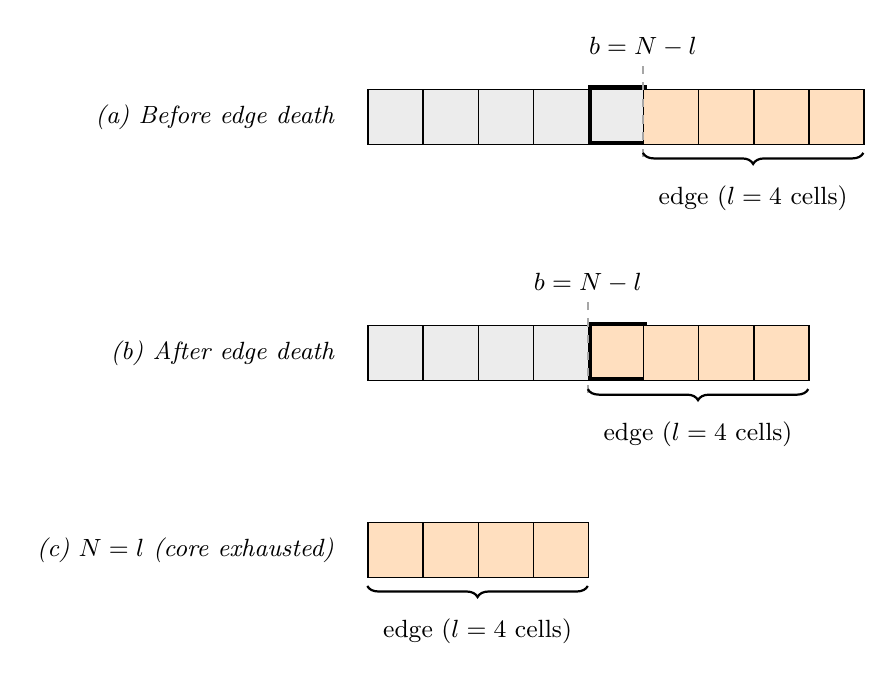
\begin{tikzpicture}[
    every node/.style={font=\small},
    cellbox/.style={draw=black, line width=0.5pt, minimum width=0.7cm, minimum height=0.7cm, anchor=south west},
    corecell/.style={cellbox, fill=gray!15},
    edgecell/.style={cellbox, fill=orange!25},
    tracked/.style={line width=1.6pt},
    bracket/.style={decorate, decoration={brace, amplitude=4pt, mirror}, thick},
    boundary/.style={dashed, gray!70, thick},
    panellabel/.style={anchor=east, font=\small\itshape},
]

% Panel (a). N = 9, l = 4, so b = 5. Tracked cell at position 4 (innermost core).
\node[panellabel] at (-0.3, 3.35) {(a) Before edge death};

\foreach \i in {0,1,2,3} {
  \node[corecell] at (\i*0.7, 3.0) {};
}
\node[corecell, tracked] at (4*0.7, 3.0) {};
\foreach \i in {5,6,7,8} {
  \node[edgecell] at (\i*0.7, 3.0) {};
}

\draw[boundary] (3.5, 2.85) -- (3.5, 4.0);
\node[above, font=\small] at (3.5, 4.0) {$b = N - l$};

\draw[bracket] (3.5, 2.9) -- (6.3, 2.9)
  node[midway, below=8pt, font=\small] {edge ($l=4$ cells)};

% Panel (b). N = 8, l = 4, so b = 4. The tracked cell, same physical
% position, has been reclassified into the edge.
\node[panellabel] at (-0.3, 0.35) {(b) After edge death};

\foreach \i in {0,1,2,3} {
  \node[corecell] at (\i*0.7, 0.0) {};
}
\node[edgecell, tracked] at (4*0.7, 0.0) {};
\foreach \i in {5,6,7} {
  \node[edgecell] at (\i*0.7, 0.0) {};
}

\draw[boundary] (2.8, -0.15) -- (2.8, 1.0);
\node[above, font=\small] at (2.8, 1.0) {$b = N - l$};

\draw[bracket] (2.8, -0.1) -- (5.6, -0.1)
  node[midway, below=8pt, font=\small] {edge ($l=4$ cells)};

% Panel (c). After enough edge deaths, N has fallen to l. The boundary
% collapses to b = 0 and the entire chain is edge.
\node[panellabel] at (-0.3, -2.15) {(c) $N = l$ (core exhausted)};

\foreach \i in {0,1,2,3} {
  \node[edgecell] at (\i*0.7, -2.5) {};
}

\draw[bracket] (0, -2.6) -- (2.8, -2.6)
  node[midway, below=8pt, font=\small] {edge ($l=4$ cells)};

\end{tikzpicture}
\caption{The conveyor belt as a consequence of recomputing the boundary, illustrated on a small didactic chain with $N = 9$ initial cells and $l = 4$. The rightmost $l$ cells (orange) form the edge; the rest (grey) form the core. (a) Before the event, the cell drawn with a heavy outline sits in the core, immediately inside the boundary $b = N - l$. (b) After an outer edge cell has died, $N$ has dropped to $8$ and the recomputed boundary has moved one position inward; the tracked cell, in the same physical position, is now part of the edge. No cell has been shuffled; the bracket has shifted over it. (c) After enough cumulative edge deaths, $N$ reaches $l$: the boundary collapses to $b = 0$, the entire chain is edge, and the dynamics enter Phase 2. An edge birth is the symmetric operation, with the boundary moving outward by one position and the innermost edge cell reclassified as core.}
\label{fig:conveyor}
\end{figure}

The conveyor belt produces two qualitatively different regimes of decline. While the core still has cells in it ($N(t) > l$), each edge death is replaced immediately by a core cell, so the edge stays at exactly $l$ cells. Only the $l$ edge cells contribute to net loss, at rate $\sE \cdot l$ per unit time, and the total population falls linearly, where $\sE = \dEdge - \bEdge$. The duration of this buffered decline is
\begin{equation}
T_1 \;=\; \frac{\Nzero - l}{\sE \cdot l},
\label{eq:T1}
\end{equation}
which is long at low dose (slow edge turnover empties the core gradually) and brief at high dose (fast edge turnover empties the core quickly). Once the core is exhausted ($N(t) \le l$; Figure~\ref{fig:conveyor}(c)), the edge is the entire remaining population, and there is no reservoir to draw on. The remaining $\le l$ cells decay exponentially at rate $\sE$, just as a well-mixed population would. The transition between these two regimes is sharp on the simulation timescale: it happens at the moment the last core cell is converted to edge. After that point, the dynamics on the chain are indistinguishable from those of a one-compartment well-mixed model with $N = l$.

\subsection{Mutations, rescue, and initial condition}
\label{ssec:mutations}

Mutations are replication-linked: at each WT birth event, with probability $\mu$, the daughter is an R cell instead of WT; otherwise the daughter inherits the parent's genotype. Mutations are irreversible (no back-mutation from R to WT), so once a lineage is R, all of its descendants are R. Because mutations ride on births, they appear at specific spatial positions on the chain (the position of the dividing parent); a mutation born deep in the core enters the world at the core's spatial location and must be physically transported to the edge to come under selection.

Every R lineage that ever appears is tagged with a unique identifier when its founder is born, and that identifier propagates to all descendants. This lets us follow each mutation individually: where it was born (core or edge), when it appeared, how its descendant population grew, whether it ever reached the edge, and whether it contributed to rescue. The per-lineage records produced by this tracking are the basis for most of the analyses in later sections.

A run is declared $\mathrm{rescued}$ when the edge contains at least $r_{\mathrm{thr}} = 10$ resistant cells simultaneously. The choice of $r_{\mathrm{thr}} = 10$ is high enough to be well past the establishment bottleneck (the regime where a small R lineage might still go extinct by chance) but small enough that rescue is declared promptly after takeover begins. Once an R lineage is past establishment in the edge, where $\sR > 0$, it grows deterministically to dominance. Every simulation terminates naturally on one of two events: rescue ($\ge r_{\mathrm{thr}}$ R cells in the edge) or extinction ($N = 0$). There are no artificial time or generation caps. Both endpoints are guaranteed by the dynamics: either a successful resistant lineage establishes in time, or the wild-type population is driven to zero. The model cannot stall in between.

Every simulation starts at $t = 0$ with $N = \Nzero$ wild-type cells and no resistant cells. Before $t = 0$ the population is at quasi-steady state, with balanced birth and death rates in both compartments ($\bEdge = \dEdge = 1$ pre-treatment in the edge, $\bCore = \dCore$ in the core), so the biofilm neither grows nor shrinks. At $t = 0$ the antibiotic switches on: the edge WT death rate jumps from $\bEdge = 1$ to its treatment value $\dEdge > 1$, and the population begins to decline. What we simulate is therefore the response of an already-mature biofilm to a step-function antibiotic challenge. Real treatments are gradual; this abstraction strips out the loading dynamics so that the rescue dynamics, the only thing we are studying, are not entangled with growth-phase or pharmacokinetic transients.

\subsection{The well-mixed reference}
\label{ssec:wm}

To say whether the biofilm helps or hurts, we need a baseline. Our baseline is a well-mixed population of the same initial size $\Nzero$, governed by the edge birth and death rates alone: every cell is drug-exposed, none are shielded. This is the standard setting for evolutionary rescue (Wilson et al., 2017), and it is the natural null model, the same biofilm with all spatial structure removed. We simulate this fully well-mixed model (essentially a one-compartment model and faithful recreation of Wilson's evolutionary rescue model). Operationally, however, the true well-mixed reference to our biofilm model is the chain model with $l \ge \Nzero$: when the edge is as wide as the entire population, no cell is ever in the core, the conveyor belt never engages, and the dynamics reduce to a one-compartment birth-death process on scalar counts. We also maintain an independent scalar-count implementation as a cross-check; the two well-mixed models agree statistically within sampling error, which serves as an internal consistency test on the chain model.


\subsection{Parameters and simulation details}
\label{ssec:params}
Unless stated otherwise, all simulations use the parameters in Table~\ref{tab:params}. Time is measured in edge generations ($\bEdge = 1$). The dose sweep covers $\dEdge \in \{1.05,\,1.1,\,1.2,\,1.4,\,1.6,\,1.9,\,2.3,\,2.8\}$. The core-activity sweep covers $\bCore \in \{0,\,0.05,\,0.1,\,0.2,\,0.4,\,0.8\}$. The edge-width sweep covers $l \in \{25,\,50,\,100,\,200,\,400\}$. Every parameter combination is run with $5{,}000$ independent seeds; the well-mixed reference is run at the same dose points with the same seed count.

\begin{table}[h!]
\centering
\small
\begin{tabular}{lll}
\toprule
Parameter & Value & Meaning \\
\midrule
$\Nzero$           & $1000$        & Initial population size \\
$l$                & $100$ (swept) & Fixed value for edge width (\# cells exposed to drug) \\
$\bEdge$           & $1.0$         & WT birth rate in edge (sets time unit) \\
$\dEdge$           & dose (swept)  & WT death rate in edge; super-MIC is $\dEdge > 1$ \\
$\bR$              & $1.0$         & R birth rate in edge \\
$\dR$              & $0.6$         & R death rate in edge ($\sR = 0.4$) \\
$\bCore = \dCore$  & $0.2$ (swept) & Core birth \& death rate ($0$ = dormant) \\
$\mu$              & $10^{-4}$     & Mutation probability per birth \\
$r_{\mathrm{thr}}$ & $10$          & Resistant edge cells required to declare rescue \\
$K$                & $\Nzero$      & Density cap for R births (see footnote, \S\ref{ssec:chain}) \\
\bottomrule
\end{tabular}
\caption{Default model parameters. The swept variables are dose ($\dEdge$), core activity ($\bCore$), and edge width ($l$).}
\label{tab:params}
\end{table}
